\documentclass[12pt]{article}

\usepackage{sbc-template}

\usepackage{graphicx,url}

\usepackage[brazil]{babel}
\usepackage[utf8]{inputenc}  

     
\sloppy

\title{Implementa\c{c}\~ao do k-nearest neighbors -- KNN\\ em VHDL}

\author{Alexandre G. da Costa\inst{1}, Diego P. Jaccottet\inst{1}, Leandro W.
  Dias\inst{1} }


\address{CDTec -- Universidade Federal de Pelotas
  (UFPEL)\\
  CEP 96.010-610 -- Pelotas -- RS -- Brazil
  \email{alexandre.costa@inf.ufpel.edu.br, \{diego.porto.j,lwdias\}@gmail.com}
}

\begin{document} 

\maketitle

\begin{abstract}
  This paper describes ...
\end{abstract}
     
\begin{resumo} 
  Este artigo descreve ...
\end{resumo}


\section{Introdu\c{c}\~ao}

O objetivo deste projeto é implementar o algoritmo KNN na placa Altera Cyclone
(2C35) FPGA de 35.000 LEs, afim de reconhecer indivíduos. Sendo que a entrada
será o esqueleto do indivíduo, esse esqueleto é inferido a partir de filmagem
tridimensional realizada pelo Kinect Versão 2 pelo seu SDK. 

\section{Kinect Vers\~ao 2} \label{sec:kinectversion2}

O Kinect é um sensor equipado de uma câmera RGB, um sensor de profundidade
composto de um emissor de luz infravermelho e uma câmera sensível à
profundidade. 

O principio básico por trás do sensor de profundidade do Kinect é a emissão
de um padrão de infravermelho e a captura simultânea da imagem desse
infravermelho com uma câmera tradicional equipada com um filtro, que permite
capturar o infravermelho e bloquear outras formas de onda. O processador de
imagens do Kinect usa as posições relativas dos pontos no padrão do
infravermelho para calcular o deslocamento da profundidade em cada posição de
pixel na imagem.

Cada pixel do mapa de profundidade representa a distância cartesiana,
em milímetros, do plano da câmera até o objeto mais próximo, naquela coordenada
(x, y) em particular. Se o valor do pixel é 0, isso indica que o sensor não
encontrou nenhum objeto no seu espaço de alcance naquela localização (x, y).
Essa projeção é mencionado como espaço de profundidade. Os valores correntes
de profundidade são as distâncias do plano da câmera, ao invés das do sensor
propriamente dito.

\section{Algoritmo KNN}

O algoritmo de aprendizado supervisionado KNN é utilizado para classificar um
objeto não rotulado, baseado no rótulo de seus vizinhos mais próximos em um
espaço de exemplos \cite{Cechinel:Disertacao:2014}. Essa proximidade é, frequentemente, baseada em uma métrica
de distância entre dois pontos, por exemplo, a distância Euclidiana. De maneira
simplificada, a regra de classificação do KNN é associar a uma amostra de
teste, o rótulo da maioria das categorias de seus ``k'' vizinhos mais próximos. 

Um conjunto de treino X consiste em n pares de vetores e rótulos, dispersos em
um espaço de classes. Dado um novo par (x; $\theta$), onde apenas a medida x é
observável, o valor de $\theta$	é estimado pela utilização dos dados contidos no
conjunto X com os vetores e rótulos já conhecidos (supervisionado). Um vetor x'
é um vizinho mais próximo de x, se segundo a Equação:

$d(x_{n}', x) = min(x_i, x) i = 1, 2, ...,n$

A distância mínima entre um vetor vizinho e o vetor testado são iguais ao 
conjunto de distâncias mínimas entre os outros vetores e o vetor testado.
Normalmente, o ``voto'' do vizinho possui um peso, de acordo com a distância do 
vetor testado e seus ``k'' vizinhos mais próximos. Assim, $\theta$ é estimado 
com o rótulo desses ``k'' vizinhos mais próximos, como mostra a Figura:

\begin{figure}[ht]
	\centering
	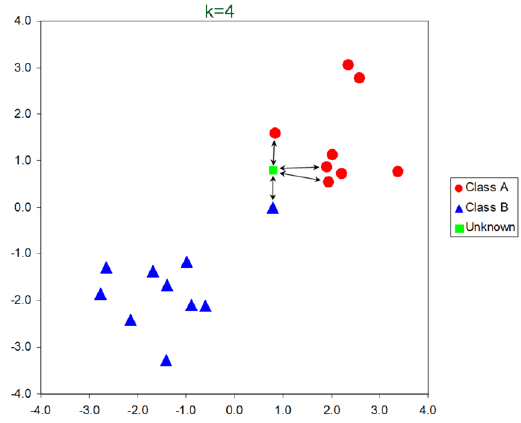
\includegraphics[width=.5\textwidth]{img/knn.png}
	\caption{Um vetor com classe desconhecida e seus 4 vizinhos}
	\label{fig:fig1}
\end{figure}

A figura mostra a representação visual de 19 vetores rotulados com classe A e B
e uma classe desconhecida. O vetor com classe desconhecida é portanto, rotulado
com seus 4 (k=4) vizinhos mais próximos de acordo com a distância euclidiana 
entre eles.

\section{Descric\~ao VHDL do Kinect vers\~ao 2}

Esta seção descreve, em VHDL, como foi implementado a comunicação do Kinect 
versão 2 com a placa Altera Cyclone (2C35) FPGA de 35.000 LEs, bem como 
aquisição dos exemplos e aquisição da imagem a ser comparada ...

\section{Descric\~ao VHDL do algoritmo KNN}

Esta seção descreve o algoritmo KNN em VHDL


\section{Conclus\~ao}\label{sec:figs}

Este trabalho desenvolveu um algoritmo em VHDL que...

%(Figure~\ref{fig:exampleFig1}), otherwise justified and indented by 0.8cm on
%both margins, as shown in Figure~\ref{fig:exampleFig2}. The caption font must

%\begin{figure}[ht]
%\centering
%\includegraphics[width=.5\textwidth]{fig1.jpg}
%\caption{A typical figure}
%\label{fig:exampleFig1}
%\end{figure}

%\begin{figure}[ht]
%\centering
%\includegraphics[width=.3\textwidth]{fig2.jpg}
%\caption{This figure is an example of a figure caption taking more than one
%  line and justified considering margins mentioned in Section~\ref{sec:figs}.}
%\label{fig:exampleFig2}
%\end{figure}

%\begin{table}[ht]
%\centering
%\caption{Variables to be considered on the evaluation of interaction
%  techniques}
%\label{tab:exTable1}
%\includegraphics[width=.7\textwidth]{table.jpg}
%\end{table}

%Bibliographic references must be unambiguous and uniform.  We recommend giving
%the author names references in brackets, e.g. \cite{knuth:84},
%\cite{boulic:91}, and \cite{smith:99}.

%The references must be listed using 12 point font size, with 6 points of space
%before each reference. The first line of each reference should not be
%indented, while the subsequent should be indented by 0.5 cm.

\bibliographystyle{sbc}
\bibliography{knn}

\end{document}
